\subsection{Unraveling the Mystery of Interference Patterns!}

\begin{tcolorbox}[colback=gray!10, colframe=black, title=E4E12] What causes interference received as a series of carriers at regular intervals across a wide frequency range?
\begin{enumerate}[label=\Alph*.]
    \item \textbf{Switch-mode power supplies}
    \item Radar transmitters
    \item Wireless security camera transmitters
    \item Electric fences
\end{enumerate} \end{tcolorbox}

\subsubsection{Explanation of the Concept}

Interference in radio communication can be caused by various electronic devices that emit electromagnetic signals. One common source of such interference is the operation of switch-mode power supplies (SMPS). These devices convert electrical power efficiently, but they can generate electromagnetic interference (EMI) due to their rapid switching action. The rapid switching creates harmonics and a series of spectral lines or carriers that can appear at regular intervals across the frequency spectrum.

\subsubsection{Understanding the Choices}

Let's analyze each of the options provided in the question:
\begin{itemize}
    \item \textbf{A. Switch-mode power supplies:} These devices are known for generating EMI, which can present as a series of interference patterns that spread across a wide frequency range.
    \item B. Radar transmitters: While they can cause interference, their signals are typically more continuous rather than discrete carriers.
    \item C. Wireless security camera transmitters: These can interfere with other devices primarily through their operating frequency but do not typically produce the same interference pattern as SMPS.
    \item D. Electric fences: They operate at low frequencies and can cause some interference, but not typically seen as series of carriers across a wide range.
\end{itemize}

Thus, option A is correct as it directly correlates with the description of the interference patterns observed in radio communications.

\subsubsection{Mathematical Insight}

To understand the interference produced by switch-mode power supplies, consider a simplified model where the switching frequency (\(f_s\)) is a known quantity. The interference signals can be modeled as harmonics of the switching frequency, defined as:

\[
f_n = n f_s
\]

for \(n = 1, 2, 3, \ldots, N\), where \(N\) is the highest harmonic of interest. The series of carriers can be calculated by determining \(f_s\) based on the device's specification (typically in kHz to MHz).

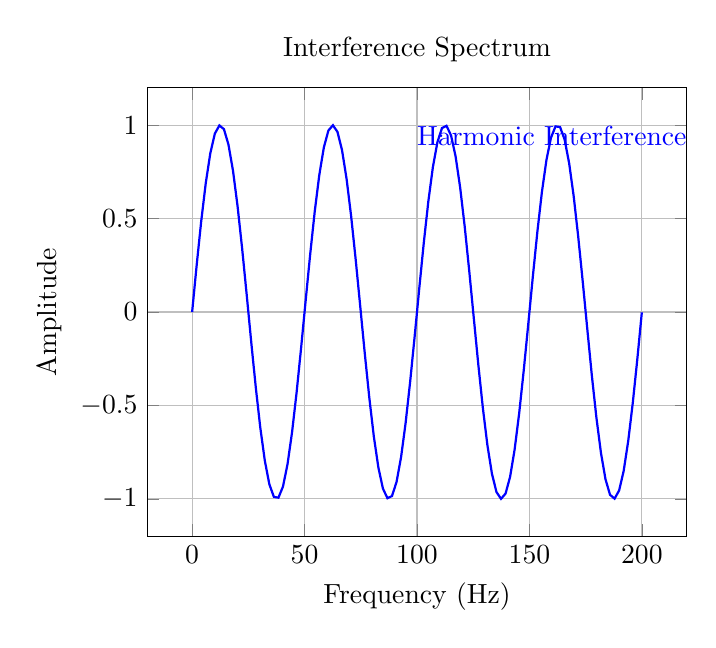
\begin{tikzpicture}
    \begin{axis}[
        title={Interference Spectrum},
        xlabel={Frequency (Hz)},
        ylabel={Amplitude},
        grid=both,
        minor grid style={gray!20},
        major grid style={gray!50},
        domain=0:200,
        samples=100
    ]
    \addplot[blue, thick] {sin(deg(2*pi*x/50))} node[pos=0.8] {Harmonic Interference};
    \end{axis}
\end{tikzpicture}

The above diagram illustrates a typical interference pattern where harmonics from the switching frequency create sinusoidal variations in amplitude, contributing to the observed interference across a wide frequency range.

In conclusion, recognizing the sources of interference and understanding the frequency behavior are essential for troubleshooting and improving radio communication systems. Knowledge of the underlying electronics, like switch-mode power supplies, helps in identifying and mitigating these interference effects effectively.
